 \documentclass[11pt]{standalone}
\usepackage{tikz}
\usetikzlibrary{calc, positioning, patterns, snakes}

\definecolor{violet}{rgb}{0.56, 0.0, 1.0}

\begin{document}
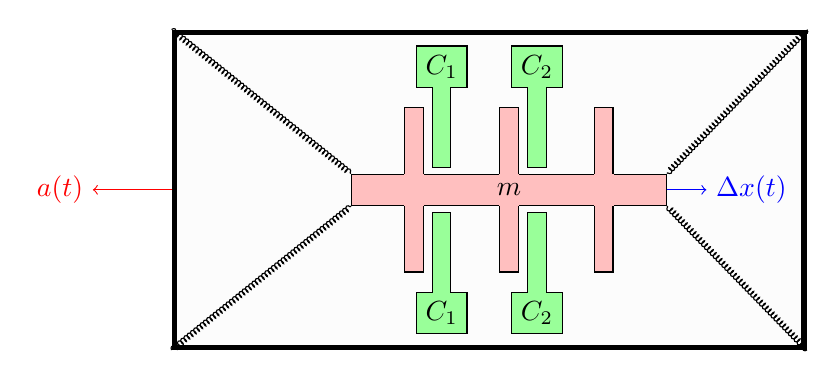
\begin{tikzpicture}
    % Define some lengths
    \def \w{8cm};
    \def \h{4cm};
    % \begin{scope}
    %     % Outer shape
    %     \node[rectangle,
    %         draw = black,
    %         % fill = lightgray,
    %         line width = 2pt,
    %         minimum width = \w,
    %         minimum height = \h] (outer) at (0,0) {};
    %     % Mass
    %     \node[rectangle,
    %         draw = black,
    %         fill = lightgray,
    %         minimum width = \w*0.5,
    %         minimum height = \h*0.1] (inner) at (0,0) {$m$};

    %     % Connect mass with fix points
    %     \draw [snake=coil, segment amplitude=1pt, segment length=1.5pt](outer.north west) -- (inner.north west);
    %     \draw [snake=coil, segment amplitude=1pt, segment length=1.5pt](outer.north east) -- (inner.north east);
    %     \draw [snake=coil, segment amplitude=1pt, segment length=1.5pt](outer.south west) -- (inner.south west);
    %     \draw [snake=coil, segment amplitude=1pt, segment length=1.5pt](outer.south east) -- (inner.south east);


    %     % Mass fingers (Electrodes connected to mass)
    %     \foreach \i in {0.2, 0.5, 0.8}
    %         {
    %             \node[rectangle,
    %                 draw = black,
    %                 fill = pink,
    %                 minimum height = .75cm,
    %                 anchor = north,
    %                 draw=black] (f1) at ($(inner.south east)!\i!(inner.south west)$) {};
    %             \node[rectangle,
    %                 draw = black,
    %                 fill = pink,
    %                 minimum height = .75cm,
    %                 anchor = south,
    %                 draw=black] (f1) at ($(inner.north east)!\i!(inner.north west)$) {};
    %         }

    %     % Fixed capacitors (Electrodes connected to fix points)
    %     \foreach \i [count=\idx] in {0.65, 0.35}
    %         {
    %             \node[rectangle,
    %                 % draw = lightgray,
    %                 fill = white!60!green,
    %                 minimum height = 1.1cm,
    %             ] (cap) at ($(inner.south east)!\i!(inner.south west) + (0, -.65)$) {};
    %             % Fixed plates at the bottom
    %             \node[rectangle,
    %                 % draw = lightgray,
    %                 fill = white!60!green,
    %                 minimum height = 0.4cm,
    %                 minimum width = 0.6cm,
    %                 anchor = north,
    %             ] (cap) at (cap.south) {$C_\idx$};
    %         }
    %     % Same for the top
    %     \foreach \i [count=\idx] in {0.65, 0.35}
    %         {
    %             \node[rectangle,
    %                 % draw = lightgray,
    %                 fill = white!60!green,
    %                 minimum height = 1.1cm,
    %             ] (cap) at ($(inner.north east)!\i!(inner.north west) + (0, .65)$) {};
    %             % Fixed plates at the bottom
    %             \node[rectangle,
    %                 % draw = lightgray,
    %                 fill = white!60!green,
    %                 minimum height = 0.4cm,
    %                 minimum width = 0.6cm,
    %                 anchor = south,
    %             ] (cap_fix) at (cap.north) {$C_\idx$};

    %         }


    %     % \draw[->, blue] ($(outer.west)!.5!(outer.north west)$) --++ (-1, 0) node[left]{$a(t)$};
    %     % \draw[->, blue] ($(r.east)!.5!(r.north east)$) --++ (1, 0) node[right]{$\Delta x(t)$};
    %     % \draw[->, red] ($(r.west)!.5!(r.south west)$) --++ (-1, 0) node[left]{$a(t)$};
    %     % \draw[->, red] ($(r.east)!.5!(r.south east)$) --++ (1, 0) node[right]{$\Delta x(t)$};
    % \end{scope}

    % In motion
    \begin{scope}[shift={(7,0)}]
        % Outer shape
        \node[rectangle,
            draw = black,
            fill = white!99!black,
            line width = 2pt,
            minimum width = \w,
            minimum height = \h] (outer) at (0,0) {};

        \begin{scope}[shift={(0.25,0)},]
            % Mass
            \node[rectangle,
                draw = black,
                fill = pink,
                minimum width = \w*0.5,
                minimum height = \h*0.1] (inner) at (0,0) {$m$};

            % Connect mass with fix points
            \draw [snake=coil, segment amplitude=1pt, segment length=1.5pt](outer.north west) -- (inner.north west);
            \draw [snake=coil, segment amplitude=1pt, segment length=1.5pt](outer.north east) -- (inner.north east);
            \draw [snake=coil, segment amplitude=1pt, segment length=1.5pt](outer.south west) -- (inner.south west);
            \draw [snake=coil, segment amplitude=1pt, segment length=1.5pt](outer.south east) -- (inner.south east);

            % Mass fingers (Electrodes connected to mass)
            \foreach \i in {0.2, 0.5, 0.8}
                {
                    \node[rectangle,
                        draw = black,
                        fill = pink,
                        minimum height = .85cm,
                        anchor = north,
                    ] (f1) at ($(inner.south east)!\i!(inner.south west) + (0,.02)$) {};
                    \node[rectangle,
                        draw = black,
                        fill = pink,
                        minimum height = .85cm,
                        anchor = south,
                    ] (f2) at ($(inner.north east)!\i!(inner.north west) - (0,.02)$) {};
                    % Remove black lines seperating fingers from shape
                    \draw[pink, thick] ([shift={(0,-.005)}]f1.north west) -- ([shift={(0,-.005)}]f1.north east);
                    \draw[pink, thick] ([shift={(0,.005)}]f2.south west) -- ([shift={(0,.005)}]f2.south east);
                    % \draw[blue] (f2.south west) -- (f2.south east);
                }
        \end{scope}
        % Fixed capacitors (Electrodes connected to fix points)
        \foreach \i [count=\idx] in {0.575, 0.425}
            {
                % Fingers at the bottom
                \node[rectangle,
                    draw = black,
                    fill = white!60!green,
                    minimum height = 1.1cm,
                ] (caplongtop) at ($(outer.south east)!\i!(outer.south west) + (0, 1.2)$) {};
                % Fixed plates at the bottom
                \node[rectangle,
                    draw = black,
                    fill = white!60!green,
                    minimum height = 0.4cm,
                    minimum width = 0.6cm,
                    anchor = north,
                ] (cap) at ($(caplongtop.south) + (0,.1)$) {$C_\idx$};
                % Same for the top (fingers)
                \node[rectangle,
                    draw = black,
                    fill = white!60!green,
                    minimum height = 1.1cm,
                ] (caplongbottom) at ($(outer.north east)!\i!(outer.north west) + (0, -1.2)$) {};
                % Fixed plates at the top
                \node[rectangle,
                    draw = black,
                    fill = white!60!green,
                    minimum height = 0.4cm,
                    minimum width = 0.6cm,
                    anchor = south,
                ] (cap) at ($(caplongbottom.north) + (0,-.1)$) {$C_\idx$};
                % Remove black lines seperating ? from fixed plates
                \draw[white!60!green, thick] ([shift={(0.015,.09)}]caplongtop.south west) -- ([shift={(-0.015,.09)}]caplongtop.south east);
                \draw[white!60!green, thick] ([shift={(0.015,-.09)}]caplongbottom.north west) -- ([shift={(-0.015,-.09)}]caplongbottom.north east);
            }

        \draw[->, red] (outer.west) --++ (-1, 0) node[left] {$a(t)$};
        \draw[->, blue] (inner.east) --++ (.5, 0) node[right]{$\Delta x(t)$};
    \end{scope}

\end{tikzpicture}

\end{document}